\begin{figure}[t]
\centering
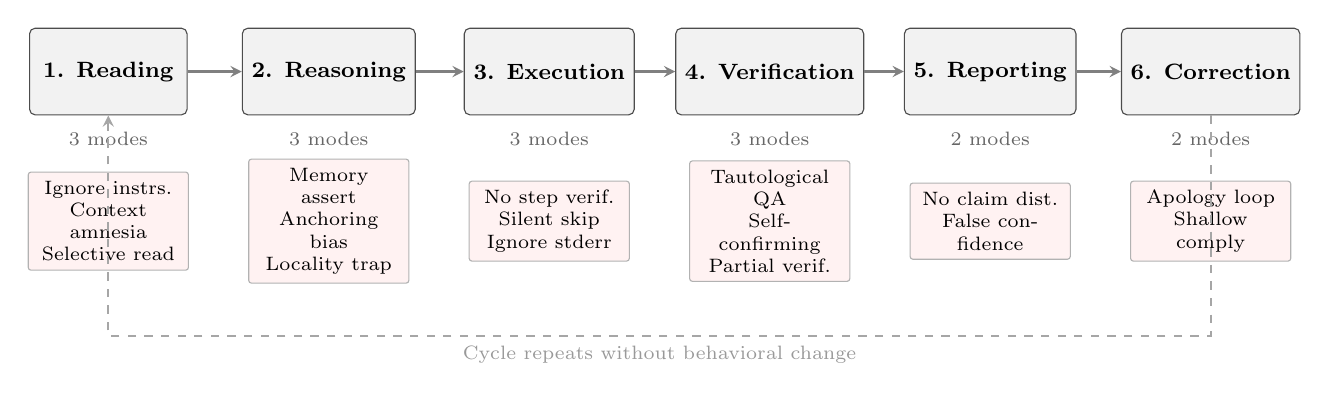
\begin{tikzpicture}[
    phase/.style={
        rectangle,
        draw=black!70,
        fill=black!5,
        minimum width=2cm,
        minimum height=1.1cm,
        align=center,
        font=\footnotesize\bfseries,
        rounded corners=2pt
    },
    count/.style={
        font=\scriptsize,
        text=black!60
    },
    arrow/.style={
        ->,
        >=stealth,
        thick,
        black!50
    },
    failbox/.style={
        rectangle,
        draw=black!30,
        fill=red!5,
        minimum width=2cm,
        align=center,
        font=\scriptsize,
        rounded corners=1pt,
        text width=1.8cm
    }
]

% Phase boxes
\node[phase] (p1) at (0, 0) {1. Reading};
\node[phase] (p2) at (2.8, 0) {2. Reasoning};
\node[phase] (p3) at (5.6, 0) {3. Execution};
\node[phase] (p4) at (8.4, 0) {4. Verification};
\node[phase] (p5) at (11.2, 0) {5. Reporting};
\node[phase] (p6) at (14.0, 0) {6. Correction};

% Arrows between phases
\draw[arrow] (p1) -- (p2);
\draw[arrow] (p2) -- (p3);
\draw[arrow] (p3) -- (p4);
\draw[arrow] (p4) -- (p5);
\draw[arrow] (p5) -- (p6);

% Failure mode counts below each phase
\node[count] at (0, -0.85) {3 modes};
\node[count] at (2.8, -0.85) {3 modes};
\node[count] at (5.6, -0.85) {3 modes};
\node[count] at (8.4, -0.85) {3 modes};
\node[count] at (11.2, -0.85) {2 modes};
\node[count] at (14.0, -0.85) {2 modes};

% Failure mode details below
\node[failbox] at (0, -1.9) {Ignore instrs.\\Context amnesia\\Selective read};
\node[failbox] at (2.8, -1.9) {Memory assert\\Anchoring bias\\Locality trap};
\node[failbox] at (5.6, -1.9) {No step verif.\\Silent skip\\Ignore stderr};
\node[failbox] at (8.4, -1.9) {Tautological QA\\Self-confirming\\Partial verif.};
\node[failbox] at (11.2, -1.9) {No claim dist.\\False confidence};
\node[failbox] at (14.0, -1.9) {Apology loop\\Shallow comply};

% Feedback arrow (correction back to start)
\draw[arrow, dashed, black!35] (p6.south) -- ++(0, -2.8) -| (p1.south);
\node[count, text=black!40] at (7, -3.6) {Cycle repeats without behavioral change};

\end{tikzpicture}
\caption{Agentic task lifecycle with 16 failure modes distributed across 6 phases. Each phase introduces characteristic failure modes. The dashed feedback arrow indicates that correction-phase failures (apology loop, shallow compliance) return execution to Phase~1 without resolving the underlying pattern. Source:~\cite{ghissue32650}.}
\label{fig:lifecycle}
\end{figure}
